\documentclass{beamer}
\usepackage{graphicx}
\usepackage{hyperref}
\usepackage{amsmath}

\title{Mixed Effects Models - Day 4}
\subtitle{Generalised Least Squares - GLS}
\author{Marieke Wesselkamp\\Department of Biometry and Environmental Systems Analysis\\Albert-Ludwigs-University of Freiburg (Germany)}
\date{February 2023}

\begin{document}

\begin{frame}
  \titlepage
\end{frame}

\begin{frame}{Ways to Avoid Mixed Effects Models}
  \begin{itemize}
    \item Ignore dependencies: simply \textbf{wrong}
    \item Take means within groups
    \item Use grouping variable as a covariate
  \end{itemize}
\end{frame}

\begin{frame}[fragile]{Taking Means Within Groups}
  \small{Taking means within groups...}
  
  \begin{verbatim}
set.seed(1)
treat <- rep(c("A", "B"), each = 20)
group <- rep(1:4, each = 10) # create a 4-block design
measurement <- rep(1:10, 4)
groupRan <- rnorm(10, 0, 1)
mean.A <- 8
mean.B <- 6
mean <- as.numeric(treat == "A") * mean.A
mean[21:40] <- mean.B
sd = 1
RE <- groupRan[group]
response <- rnorm(n = 40, mean = mean, sd = 1) + RE
example_2 <- data.frame(treat, group, measurement, response)
example_2$group <- as.factor(example_2$group)
attach(example_2)
  \end{verbatim}
\end{frame}

\begin{frame}{Boxplot of Response by Group}
  \begin{center}
    \includegraphics[width=0.5\textwidth]{boxplot_response_by_group} % Replace with actual path to plot
  \end{center}
  \smallskip
  \textbf{Reduction of 40 data points to 4.}
\end{frame}

\begin{frame}[fragile]{Analysis of Variance (ANOVA)}
  \small{...provides less information and power than accounting for random effects.}
  \begin{verbatim}
means <- data.frame(
  treat = c(rep("A",2),rep("B",2)), 
  response = c(tapply(response, group, mean))
)
summary(aov(response ~ treat, means))
  \end{verbatim}
\end{frame}

\begin{frame}[fragile]{Using Grouping as a Fixed Covariate}
  \small{Using grouping as a fixed covariate...}
  
  \begin{center}
    \includegraphics[width=0.5\textwidth]{boxplot_response_fixed_covariate} % Replace with actual path to plot
  \end{center}
  
  \begin{verbatim}
summary(aov(response ~ treat + group))
  \end{verbatim}
  \small{...uses too many degrees of freedom.}
\end{frame}

\begin{frame}{Issues with Avoiding Mixed Effects Models}
  \small{All these Mixed Effects Models avoidance mechanisms have \textbf{issues}.}
  \begin{quote}
    Generalised Least Squares can be a solution.
  \end{quote}
\end{frame}

\begin{frame}{The Linear Model}
  Remember the Linear Model:
  \[
  \mathbf{y} = \mathbf{X} \cdot \mathbf{b} + \mathbf{e}, \quad \epsilon \sim \mathcal{N}(0, \sigma^2_{e} \cdot \mathbf{I})
  \]
  And the residual variance-covariance matrix in a linear model:
  \[
  \mathbf{V} = \sigma^2 \cdot \mathbf{I} = 
  \begin{bmatrix}
  \sigma^2 & 0 & \cdots & 0 \\
  0 & \sigma^2 & \cdots & 0 \\
  \vdots & \vdots & \ddots & \vdots \\
  0 & 0 & \cdots & \sigma^2
  \end{bmatrix}
  \]
\end{frame}

\begin{frame}{Covariance Matrix}
  The off-diagonals tell the covariance $covar_{ij}$ between $y_i$ and $y_j$:
  \[
  \mathbf{V} = 
  \begin{bmatrix}
  \sigma^2 & 0 & \cdots & 0 \\
  0 & \sigma^2 & \cdots & 0 \\
  \vdots & \vdots & \ddots & \vdots \\
  0 & 0 & \cdots & \sigma^2
  \end{bmatrix}
  \]
  Defined as $0$ for \textit{independent} data.
\end{frame}

\begin{frame}{Generalised Least Squares (GLS)}
  Generalised least squares (GLS) estimation allows to \textbf{explicitly} work with the variance-covariance matrix $\mathbf{V_i}$ of the residuals within a group.
  \begin{itemize}
    \item Different $\sigma^2$ on the diagonals to account for heteroscedasticity
    \item Off-diagonals for non-independency
  \end{itemize}
  \begin{quote}
    This means errors are not $iid$ distributed anymore.
  \end{quote}
\end{frame}

\begin{frame}[fragile]{R Code Setup for GLS}
  \begin{verbatim}
repeated <- read.table("repeated.txt", header = TRUE)
repmeasures <- read.table("repmeasures.txt", header = TRUE)
farms <- read.table("farms.txt", header = TRUE)
farms$farm <- factor(farms$farm)
fertilizer <- read.table("fertilizer.txt", header = TRUE)
blowfly <- read.table("blowfly.txt", header = TRUE)
blowfly$flies <- as.numeric(blowfly$flies)
blowfly$week <- c(1:362)
blowfly <- na.omit(blowfly)
library(lattice)
library(nlme)
  \end{verbatim}
\end{frame}

\begin{frame}{Marginal Model}
  This gives us the Marginal Model:
  \[
  \mathbf{y} = \mathbf{X} \cdot \mathbf{b} + \mathbf{e}, \quad \epsilon \sim \mathcal{N}(0, \mathbf{V_i})
  \]
  The \textbf{marginal model} describes the deterministic part for the average trend in the data while considering the correlation between non-independent data within a group.
\end{frame}

\begin{frame}{Properties of Marginal Model}
  \begin{itemize}
    \item In the Marginal Model fitted with GLS, there are \textbf{NO} random effects.
    \item The Marginal Model ignores the random structure due to grouping and fits directly to the deterministic trend.
  \end{itemize}
  \begin{quote}
    You won't get among- or within-group variances or group-specific (random) intercepts and slopes.
  \end{quote}
\end{frame}

\begin{frame}{Specifying the Covariance Matrix}
  All that matters is in the a-priori specified residual variance-covariance matrix.
  We will continue working with the assumption of homoscedasticity (identically distributed residual variances $\sigma^2$) but will work with different error structures on the off-diagonals.
  \[
  \mathbf{V_i} = 
  \begin{bmatrix}
  \sigma^2 & c_{12} & c_{13} & c_{14} & c_{15} \\
  c_{21} & \sigma^2 & c_{22} & c_{23} & c_{24} \\
  c_{31} & c_{32} & \sigma^2 & c_{34} & c_{35} \\
  c_{41} & c_{42} & c_{43} & \sigma^2 & c_{45} \\
  c_{51} & c_{52} & c_{53} & c_{54} & \sigma^2
  \end{bmatrix}
  \]
\end{frame}

\begin{frame}{Correlation Matrix in GLS}
  In practice, GLS works with the correlation instead of the variance-covariance matrix.
  \[
  \text{cor}(y_i,y_j) = \frac{\text{cov}(y_i, y_j)}{\sqrt{\text{var}(y_i)} \cdot \sqrt{\text{var}(y_j)}}
  \]
  This makes the variance-covariance matrix a correlation matrix:
  \[
  \mathbf{V_i} = 
  \begin{bmatrix}
  1 & \rho_{12} & \rho_{13} & \rho_{14} & \rho_{15} \\
  \rho_{21} & 1 & \rho_{23} & \rho_{24} & \rho_{25} \\
  \rho_{31} & \rho_{32} & 1 & \rho_{34} & \rho_{35} \\
  \rho_{41} & \rho_{42} & \rho_{43} & 1 & \rho_{45} \\
  \rho_{51} & \rho_{52} & \rho_{53} & \rho_{54} & 1
  \end{bmatrix}
  \]
\end{frame}

\begin{frame}{Specifying Variance Structures}
  \textbf{Types of Variance Structures}
  \begin{itemize}
    \item General structure
    \item Compound symmetry
    \item Temporal or spatial autocorrelation structures
  \end{itemize}
\end{frame}

\begin{frame}{General Structure}
  \textbf{General Structure}
  
  Each element above (below) the diagonal has to be estimated: here 10 values.
  \[
  \mathbf{V_i} = 
  \begin{bmatrix}
  1 & \rho_{12} & \rho_{13} & \rho_{14} & \rho_{15} \\
  \rho_{21} & 1 & \rho_{22} & \rho_{23} & \rho_{24} \\
  \rho_{31} & \rho_{32} & 1 & \rho_{34} & \rho_{35} \\
  \rho_{41} & \rho_{42} & \rho_{43} & 1 & \rho_{45} \\
  \rho_{51} & \rho_{52} & \rho_{53} & \rho_{54} & 1
  \end{bmatrix}
  \]
  But with just one more measurement, it would already be 15 values.
  \begin{quote}
    The general structure of $\mathbf{V_i}$ is flexible but data hungry!
  \end{quote}
\end{frame}

\begin{frame}{Compound Symmetry}
  \textbf{Compound Symmetry}
  
  There is only one element to be estimated.
  \[
  \mathbf{V_i} = 
  \begin{bmatrix}
  1 & \rho & \rho & \rho & \rho \\
  \rho & 1 & \rho & \rho & \rho \\
  \rho & \rho & 1 & \rho & \rho \\
  \rho & \rho & \rho & 1 & \rho \\
  \rho & \rho & \rho & \rho & 1
  \end{bmatrix}
  \]
  \begin{quote}
    A compound symmetric $\mathbf{V_i}$ is the simplest form...but also sometimes the least appropriate form.
  \end{quote}
\end{frame}

\begin{frame}{Compound Symmetry - Suitability}
  \small{
    The compound symmetry structure is suitable for cases where repeated measurements are \textbf{not ordered} in time or space, i.e., each value in a group is \textbf{equally} correlated with each other value. For example, in the \textit{Bloodworm} feeding experiment.
  }
  \begin{center}
    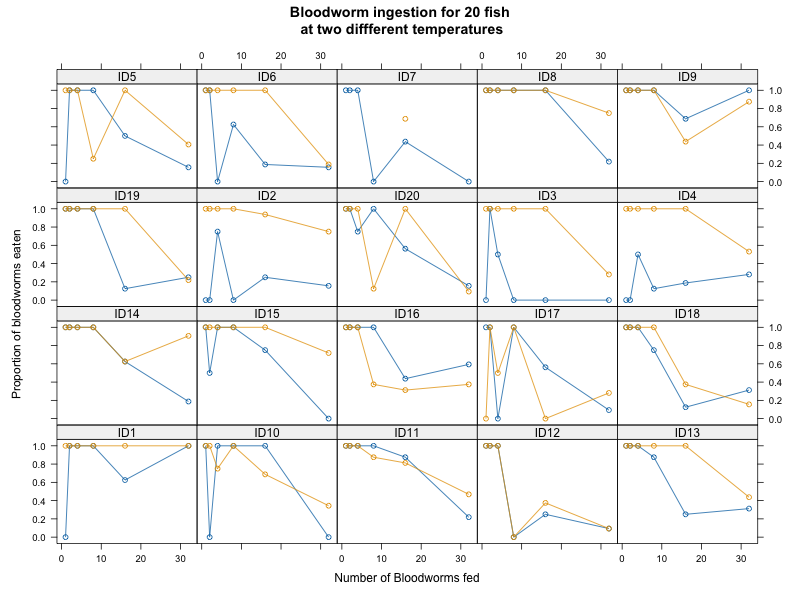
\includegraphics[width=0.4\textwidth]{bloodworms.png}
  \end{center}
\end{frame}

\begin{frame}{Temporal Autocorrelation}
  \textbf{Temporal Autocorrelation}
  
  Temporal autocorrelation matters in experiments like this where similarity between data points is not experimentally broken up but is actually carrying biological information, e.g., about the time-lag of density dependence:
  \small{For example, in the \textit{Mites} population experiment:}
  \begin{center}
    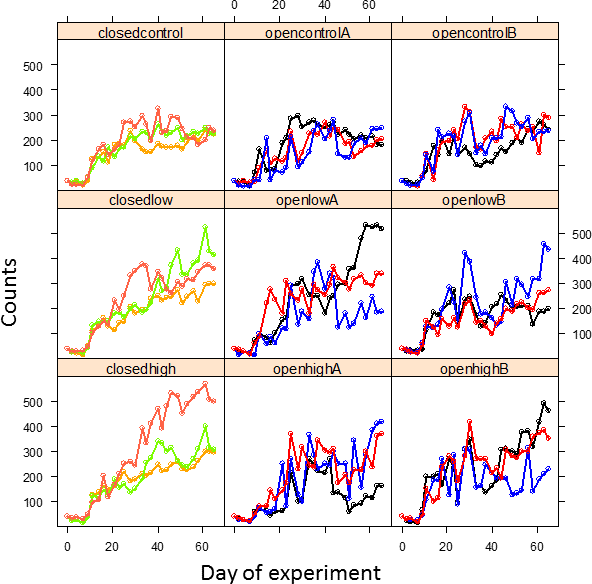
\includegraphics[width=0.4\textwidth]{counts.png}
  \end{center}
\end{frame}

\begin{frame}{Temporal or Spatial Autocorrelative Structure}
  \textbf{Temporal or Spatial Autocorrelative Structure}
  
  Allows the residuals of different time or space points to be correlated to each other, following rules given by the specified autocorrelation function.
  \begin{itemize}
    \item AR-1 autocorrelation
    \item ARMA autocorrelation
  \end{itemize}
\end{frame}

\begin{frame}{AR-1 Temporal Autocorrelation}
  \textbf{AR-1 Temporal Autocorrelation}
  
  \[
  \epsilon_t = \rho \cdot \epsilon_{t-1} + \eta_t
  \]
  \[
  \text{cor}(\epsilon_s, \epsilon_t) = 
  \begin{cases}
    1 & \text{if } s = t \\
    \rho^{\vert t-s \vert} & \text{if } s \neq t
  \end{cases}
  \]
  \begin{quote}
    Decline of relatedness with time.
  \end{quote}
\end{frame}

\begin{frame}[fragile]{Plotting AR-1 Temporal Autocorrelation}
  \begin{verbatim}
par(las = 1, pty = "s", tcl = 0.5, mgp = c(3.5,0.5,0))
a <- c(1, 0.5, 0.5^2, 0.5^3, 0.5^4, 0.5^5)
b <- c(1,2,3,4,5,6)
plot(b, a, type = "n", xlab = "time lag", ylab = "autocorrelation")
for (i in 1:6){
  arrows(b[i], 0, b[i], a[i], length = 0, lwd = 3, col = "darkred")
}
  \end{verbatim}
  \begin{center}
    \includegraphics[width=0.5\textwidth]{ar1_temporal_autocorrelation} % Replace with actual path to plot
  \end{center}
\end{frame}

\begin{frame}{AR-1 Correlation Matrix}
  From the AR-1 structure follows this correlation matrix:
  \[
  \mathbf{V_i} = 
  \begin{bmatrix}
  1 & \rho & \rho^2 & \rho^3 & \rho^4 \\
  \rho & 1 & \rho & \rho^2 & \rho^3 \\
  \rho^2 & \rho & 1 & \rho & \rho^2 \\
  \rho^3 & \rho^2 & \rho & 1 & \rho \\
  \rho^4 & \rho^3 & \rho^2 & \rho & 1
  \end{bmatrix}
  \]
\end{frame}

\begin{frame}{ARMA(p,q)-Autocorrelation}
  \textbf{ARMA(p,q)-Autocorrelation}
  
  An AR moving average model where $p$ gives the number of time points before $t$ considered for estimating the correlation of $t$ with the $t - p$ data points. $q$ gives the number of moving average parameters. ARMA(1,0) refers to the AR-1 model.
  
  ARMA(3, 0) gives:
  \[
  \epsilon_t = \phi_1\epsilon_{t-1} + \phi_p\epsilon_{t-2} + \phi_p\epsilon_{t-3}
  \]
  \begin{quote}
    Very flexible as p and/or q increases, but also gets very data-hungry!
  \end{quote}
\end{frame}

\begin{frame}{Spatial Autocorrelations}
  \begin{center}
    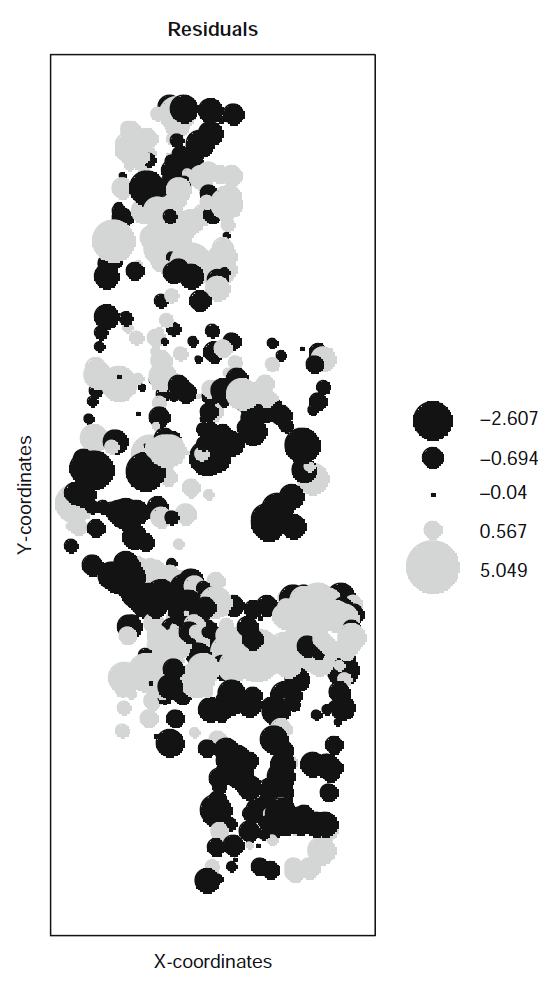
\includegraphics[width=0.75\textwidth]{spatial_residuals.png}
  \end{center}
  \small{Negative and positive residuals clump together in space.}
\end{frame}

\begin{frame}{Shown by a Variogram}
  \begin{itemize}
    \item Decay of similarity with distance between points.
    \item The "range" of a variogram is the point at which the curve levels off, i.e., the maximum distance at which data are autocorrelated.
    \item The "sill" is the spatial autocorrelation (SAC) that occurs at a distance equal to the range.
  \end{itemize}
  \begin{center}
    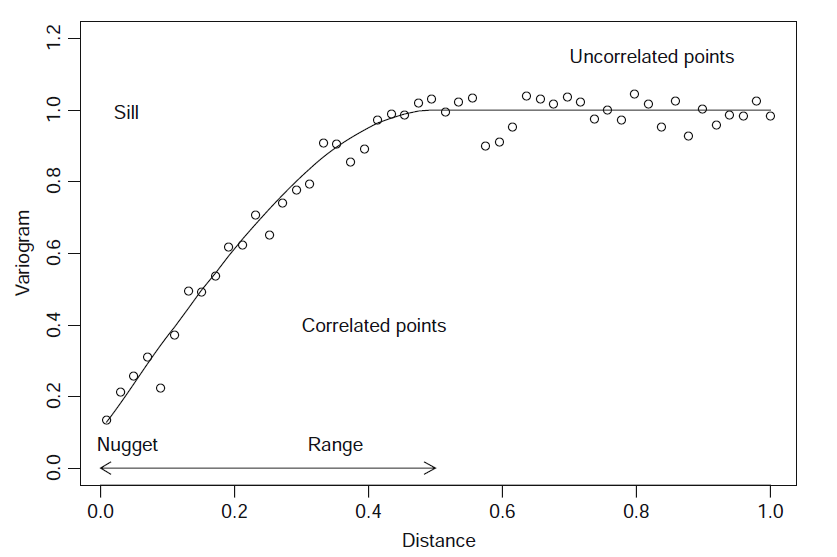
\includegraphics[width=\textwidth]{variogramm.png} % Replace with actual path to image
  \end{center}
\end{frame}

\begin{frame}{Further Reading}
  See for example Chapter 7 in: \\
  \textbf{Zuur et al.} \emph{Mixed Effects Models and Extensions in Ecology with R} \\
  \href{http://highstat.com/index.php/mixed-effects-models-and-extensions-in-ecology-with-r}{Link to book}
\end{frame}

\begin{frame}{GLS Examples}
  \begin{center}
    \textbf{GLS Examples}
  \end{center}
\end{frame}

\begin{frame}[fragile]{Example 1: Blowfly Density as a Function of Time}
  \begin{verbatim}
par(las = 1, pty = "s", tcl = 0.5, mgp = c(3.5,0.5,0))
plot(flies ~ week, blowfly, type = "l")
  \end{verbatim}
\end{frame}

\begin{frame}[fragile]{Ignoring Possible Correlation Structure}
  \begin{verbatim}
library(nlme) # contains gls
bf <- gls(flies ~ poly(week,2), na.omit(blowfly))
summary(bf)
  \end{verbatim}
  \begin{center}
    \includegraphics[width=0.5\textwidth]{plot_gls_fitted} % Replace with actual path to plot
  \end{center}
\end{frame}

\begin{frame}[fragile]{Fitting an AR(1) Model}
  Using a simple lag-1 autocorrelation model of type AR1:
  \begin{verbatim}
bf.1 <- gls(flies ~ poly(week,2), blowfly, correlation = corAR1(form = ~ week))
summary(bf.1)
  \end{verbatim}
  \begin{center}
    \includegraphics[width=0.5\textwidth]{plot_gls_ar1} % Replace with actual path to plot
  \end{center}
\end{frame}

\begin{frame}[fragile]{Auto-Correlation Function (ACF) and Partial ACF}
  A visual detection tool to detect (partial) auto-correlation of residuals.
  \begin{verbatim}
acf(residuals(bf))
pacf(residuals(bf))
  \end{verbatim}
  Difference between acf and pacf: \\
  \href{https://stats.stackexchange.com/questions/483383/difference-between-autocorrelation-and-partial-autocorrelation}{Link to explanation}
\end{frame}

\begin{frame}[fragile]{Fitting an ARMA(2,2) Model}
  Using a complex moving average autoregressive model of type ARMA(2, 2):
  \begin{verbatim}
bf.2 <- gls(flies ~ poly(week,2), blowfly, correlation = corARMA(form = ~ week, p = 2, q = 2))
summary(bf.2)
  \end{verbatim}
  \begin{center}
    \includegraphics[width=0.5\textwidth]{plot_gls_arma} % Replace with actual path to plot
  \end{center}
\end{frame}

\begin{frame}[fragile]{Model Comparison: Likelihood Ratio Test}
  The fitted models look very similar - is there really a difference? Compare the likelihood ratios.
  \begin{verbatim}
anova(bf, bf.1, bf.2) # LRT test says that there is a difference between the AR1 and ARMA(2,2) model
  \end{verbatim}
  Yes, there is.
\end{frame}

\begin{frame}[fragile]{ACF and PACF for ARMA(2,2)}
  \begin{verbatim}
acf(residuals(bf.2))
pacf(residuals(bf.2))
  \end{verbatim}
\end{frame}

\begin{frame}[fragile]{Example 2: A Fertilizer Experiment}
  \begin{verbatim}
xyplot(root ~ week|fertilizer, group = plant, fertilizer, type ="l")
  \end{verbatim}
\end{frame}

\begin{frame}[fragile]{GLS Without Correlation}
  Again, first without any correlation due to plant:
  \begin{verbatim}
model.1 <- gls(root ~ week * fertilizer, fertilizer)
summary(model.1)
  \end{verbatim}
  \begin{center}
    \includegraphics[width=0.5\textwidth]{plot_gls_no_correlation} % Replace with actual path to plot
  \end{center}
\end{frame}

\begin{frame}[fragile]{GLS with Compound Symmetry Correlation}
  Now testing a compound symmetry correlation due to "plant":
  \begin{verbatim}
model.2 <- gls(root ~ week * fertilizer, fertilizer, correlation = corCompSymm(form = ~ week|plant))
summary(model.2)
anova(model.1, model.2)
getVarCov(model.2)
cov2cor(getVarCov(model.2))
  \end{verbatim}
\end{frame}

\begin{frame}[fragile]{Model Comparison with General Structure}
  Use the most complex *general structure* matrix $\mathbf{V_i}$ and look at the correlation part of the output:
  \begin{verbatim}
model.3 <- gls(root ~ week * fertilizer, fertilizer, correlation = corSymm(form = ~ 1|plant))
summary(model.3)
getVarCov(model.3)
cov2cor(getVarCov(model.3))
anova(model.1, model.2, model.3)
  \end{verbatim}
\end{frame}

\begin{frame}[fragile]{Model Diagnostics}
  \begin{verbatim}
plot(model.3)
qqplot(rnorm(60,0,1), as.vector(residuals(model.3)))
  \end{verbatim}
\end{frame}

\begin{frame}{Recapitulation Day 4}
  After today you should know and understand:
  \begin{itemize}
    \item How a **the residual variance-covariance matrix** encodes the assumption of correlation between data points within a group.
    \item What the **off-diagonals** in a residual covariance matrix are.
    \item The **assumption** of linear models that is relaxed in GLS.
    \item The difference between **general**, **compound symmetric**, and various forms of **temporal autocorrelation** correlation matrices (AR1, ARMA(p, q)).
  \end{itemize}
  \textbf{Exercises today}: Exercises on GLS. Prepare for tomorrow. Read and discuss paper on Ilias.
\end{frame}

\end{document}
